\ifdefined\ishandout
\documentclass[handout]{beamer}
\else
\documentclass{beamer}
\fi

\usepackage[frenchb]{babel}
\usepackage[T1]{fontenc}
\usepackage[latin1]{inputenc}
\usepackage{hyperref}
\usepackage{multirow}
\usepackage{listings}
\usepackage{fancyvrb}
\usepackage{tikz}
\usepackage{framed}
\usepackage{algorithm}
\usepackage{algorithmic}
\usepackage{xcolor}
\usepackage{color, colortbl}
\ifdefined\ishandout
\usepackage{handoutWithNotes}
\fi
\usepackage{slashbox}
\usepackage{amsmath}
\usepackage{bm}
\usepackage{hhline}

\usetikzlibrary{shapes.geometric}
\usetikzlibrary{positioning}
\usetikzlibrary{shapes.arrows, chains}
\usetikzlibrary{arrows,calc}
\usetikzlibrary{shapes.multipart}
\usepackage{array}
\usetheme{Boadilla}

\usefonttheme[onlymath]{serif}

\newcommand{\R}{\mathbb{R}}
\newcommand{\C}{\mathbb{C}}
\newcommand{\N}{\mathbb{N}}
\newcommand{\Z}{\mathbb{Z}}
\newcommand{\E}{\mathbb{E}}
\newcommand{\Var}{\text{Var}}
\newcommand{\Cov}{\text{Cov}}
\ifdefined\ishandout
\pgfpagesuselayout{3 on 1 with notes}[a4paper,border shrink=5mm]
\usecolortheme{dove}
\else
%\usecolortheme{dolphin}
\usecolortheme{beaver}
\fi


\lstnewenvironment{codeC}
{ \lstset{language=C,
    otherkeywords={printf,scanf}}
}
{}

\ifdefined\ishandout
\definecolor{mygreen}{rgb}{0,0,0}
\definecolor{mymauve}{rgb}{0,0,0}
\definecolor{myblue}{rgb}{0,0,0}
\else
\definecolor{mygreen}{rgb}{0,0.6,0}
\definecolor{mymauve}{rgb}{0.58,0,0.82}
\definecolor{myblue}{rgb}{0,0,1}

\fi

%% Notes
%\setbeameroption{show only notes}


\definecolor{mygray}{rgb}{0.5,0.5,0.5}

\lstset{ language=Python,%
  backgroundcolor=\color{white},   % choose the background color; you must add \usepackage{color} or \usepackage{xcolor}
  basicstyle=\footnotesize,        % the size of the fonts that are used for the code
  breakatwhitespace=false,         % sets if automatic breaks should only happen at whitespace
  breaklines=true,                 % sets automatic line breaking
  captionpos=b,                    % sets the caption-position to bottom
  commentstyle=\color{mygreen},    % comment style
  deletekeywords={...},            % if you want to delete keywords from the given language
  escapeinside={\%*}{*)},          % if you want to add LaTeX within your code
  extendedchars=true,              % lets you use non-ASCII characters; for 8-bits encodings only, does not work with UTF-8
  frame=tb,	                   % adds a frame around the code
  keepspaces=true,                 % keeps spaces in text, useful for keeping indentation of code (possibly needs columns=flexible)
  keywordstyle=\color{blue},       % keyword style
  otherkeywords={*,...},           % if you want to add more keywords to the set
  numbers=none,                    % where to put the line-numbers; possible values are (none, left, right)
  numbersep=5pt,                   % how far the line-numbers are from the code
  numberstyle=\tiny\color{mygray}, % the style that is used for the line-numbers
  rulecolor=\color{black},         % if not set, the frame-color may be changed on line-breaks within not-black text (e.g. comments (green here))
  showspaces=false,                % show spaces everywhere adding particular underscores; it overrides 'showstringspaces'
  showstringspaces=false,          % underline spaces within strings only
  showtabs=false,                  % show tabs within strings adding particular underscores
  stepnumber=2,                    % the step between two line-numbers. If it's 1, each line will be numbered
  stringstyle=\color{mymauve},     % string literal style
  tabsize=3,	                   % sets default tabsize to 2 spaces
  title=\lstname                   % show the filename of files included with \lstinputlisting; also try caption instead of title
}
%\lstset{language=Python,
% breakatwhitespace=false,         % sets if automatic breaks should only happen at whitespace
%  breaklines=true,                 % sets automatic line breaking
%  captionpos=b,                
%%commentstyle=\itshape\color{mymauve},
%%keywordstyle=\bfseries\color{myblue},
%numbers=left,                    % where to put the line-numbers; possible values are (none, left, right)
%  numbersep=8pt,                   % how far the line-numbers are from the code
%  numberstyle=\tiny\color{mygray}, % the style that is used for the line-numbers
%%  rulecolor=\color{black},         % if not set, the frame-color may be changed on line-breaks within not-black text (e.g. comments (green here))
%  showspaces=false,                % show spaces everywhere adding particular underscores; it overrides 'showstringspaces'
%%  showstringspaces=false,          % underline spaces within strings only
%  showtabs=false,                  % show tabs within strings adding particular underscores
%  stepnumber=2,                    % the step between two line-numbers. If it's 1, each line will be numbered
%%  stringstyle=\color{mygreen},     % string literal style
%  tabsize=2 
%}
\ifdefined\ishandout
\newcommand{\red}{\textbf}
\else
\newcommand{\red}{\textcolor{red}}
\fi
%\newcommand \emph
%Default size : 12.8 cm * 9.6 cm

\newcommand{\tmark}[1]{\tikz[remember picture, baseline=-.5ex]{\coordinate(#1);}}

\ifdefined\ishandout
\newenvironment<>{codeblock}[1]{%begin
  \setbeamercolor{block title}{fg=black,bg=lightgray!80}%
  \begin{block}{#1}}
  % \begin{codeC}}
  %  {\end{codeC}
{  
\end{block}}

\newenvironment<>{termblock}[1]{
    \setbeamercolor{block title}{fg=black,bg=lightgray!90}%
    \begin{block}{#1}
}
%     \begin{Verbatim}}
{%\end{Verbatim}
\end{block}
}

\definecolor{bluegreen}{RGB}{0,0,0}
%\definecolor{bluegreen}{rgb}{0,0.6,0.8}
\else

\newenvironment<>{codeblock}[1]{%begin
  \setbeamercolor{block title}{fg=darkgray,bg=yellow}%
  \begin{block}{#1}}
  % \begin{codeC}}
  %  {\end{codeC}
{  
\end{block}}

\newenvironment<>{termblock}[1]{
    \setbeamercolor{block title}{fg=white,bg=lightgray}%
    \begin{block}{#1}}
%     \begin{Verbatim}}
{%\end{Verbatim}
\end{block}
}

\definecolor{bluegreen}{RGB}{0,149,182}
%\definecolor{bluegreen}{rgb}{0,0.6,0.8}
\fi

%\newcommand{\output}[1]{
\setbeamertemplate{navigation symbols}{}
\newcommand{\bvrb}{\Verb[commandchars=£µ§,formatcom=\color{bluegreen}]}
\newcommand{\footvrb}{\footnotesize\Verb}
\newcommand{\vrbalert}[2][]{\visible<#1>{#2}}
%%% Commande pour les listes/arbres
\newcommand{\mvide}{\nodepart{one} \nodepart{two}}
\newcommand{\tvide}{\nodepart{one} \nodepart{two} \nodepart{three}}

%%Fin des commandes pour les listes/arbres.



%%% Paramètres du cours (à régler)
%Numéro du cours
\newcommand{\nb}{1}

\title[Linear Algebra]{Probabilities/Statistics}
\author[]{julien.brajard@upmc.fr}
\institute[UPMC]{UPMC}
\date{1-5 August 2016}
\begin{document}
%%%%%%%%%%%%%%%%%%%%% SLIDES DE TITRE
\begin{frame}
\titlepage
%\centering{
%\url{http://australe.upmc.fr} (onglet EPU-C5-IGE Info Gen)}
\end{frame}
%%%%%%%%%%%%%%%%%%%%%

\begin{frame}
\frametitle{What is a probability ?}
\framesubtitle{An oversimplified explanation}
\begin{block}{A attempt of definition}
Let us consider a random event $\mathcal{E}$, which can possibly occure among
a set of possible events.

The \alert{probability} of this event is a "measure" of "how likely" this event can occure.
The probability is denoted $P(\mathcal{E})$ and is between $0$ for impossible event to $1$ for
a certain event.
\end{block}
Some examples:
\begin{itemize}
\item A birth can be a boy or a girl. $P(\text{being a boy})=0.5$, $P(\text{being a girl})=0.5$.
\item The probability for a random picked up person in the population to be taller than 1m80.
\end{itemize}
\alert{Be careful}: The set of possible events is crucial.
\begin{itemize}
\item If you play to the lottery, $P(\text{win})\approx \frac{1}{14000000}$
\item If you don't play to the lottery, $P(\text{win})=0$
\end{itemize}
\end{frame}

%%%%%%%%%%%%%%%%%%%%%%%%%%%%%%%%%%%%%%%%%%%%%%%%%%%%%%%%%%%%%%%%%%%%%%%%%%%%%%%%%%%%%%

\begin{frame}
\frametitle{Some properties of the probability}
Let us denote $\Omega$ the set of possible events. $A$,$B$ are events $\in \Omega$.

\begin{itemize}
\item $P(\Omega)=1$
\item $P(A\cup B)=P(A)+P(B) - P(A \cap B)$
\item $P(\text{not}A)= 1 - P(A)$
\item $P(A|B)$ is probability of $A$ knowing B
\end{itemize}

\begin{block}{Definition}
Two events $A$ and $B$ are said to be \alert{independant} if:
and only if
$$P(A\cap B)=P(A)\times P(B)$$
\end{block}
\note{draw diagrams}
\end{frame}


%%%%%%%%%%%%%%%%%%%%%%%%%%%%%%%%%%%%%%%%%%%%%%%%%%%%%%%%%%%%%%%%%%%%%%%%%%%%%%%%%%%%%%


\begin{frame}
\frametitle{Random variable}
\begin{block}{Definition (intuitive)}
A \alert{random variable} is a variable that can take randomly different values.
\end{block}
A random variable can be:
\begin{itemize}
\item Discrete
\begin{exampleblock}{Ex. 1: Value of a dice}
The result $X$ of a dice roll is a random variable with values in $\{1,2,3,4,5,6\}$.
\end{exampleblock}
\item Continuous
\begin{exampleblock}{Ex. 2: Sea temperature}
The temperature of the sea for this afternoon at 2 p.m. is a random value in $
\R$.
\end{exampleblock}
\end{itemize}
\end{frame}


%%%%%%%%%%%%%%%%%%%%%%%%%%%%%%%%%%%%%%%%%%%%%%%%%%%%%%%%%%%%%%%%%%%%%%%%%%%%%%%%%%%%%%
\begin{frame}
\frametitle{Probability distribution}
The value or the range of values taken by a random variable is a random event.
The probability distribution describes the probability of all the values taken by a random
variable. The way to describe it depends if the variable is continue or discrete:
\begin{itemize}
\item for discrete variables: the \alert{Probability Mass Function}
\item for continuous variables: the \alert{Probability Density Function}
\end{itemize}
\end{frame}


%%%%%%%%%%%%%%%%%%%%%%%%%%%%%%%%%%%%%%%%%%%%%%%%%%%%%%%%%%%%%%%%%%%%%%%%%%%%%%%%%%%%%%
\begin{frame}
\frametitle{Probability Mass Function}
Given a discrete random variable $X$, the Probability Mass function $P$ gives 
the probability of each state possibility taken by $X$. 

This probability is denoted $P(x)$ or 
more clearly $P(X=x)$. 

Note that $ \sum_x P(X=x) = 1 $
\begin{exampleblock}{Example 1:one dice roll}
$P(X=x) = \frac{1}{6}$ (uniform distribution)
\end{exampleblock}

\begin{exampleblock}{Example 2: the sum of two dice rolls}
\begin{tabular}{|c|c|c|c|c|c|c|c|c|c|c|c|}
\hline
$x$ & $2$ & $3$ & $4$ & $5$ & $6$ & $7$ & $8$ & $9$ & $10$ & $11$ & $12$ \\
\hline
$P(X=x)$& $\frac{1}{36}$ &  $\frac{2}{36}$ &  $\frac{3}{36}$ & $\frac{4}{36}$ &
 $\frac{5}{36}$ &  $\frac{6}{36}$ &  $\frac{5}{36}$ &  $\frac{4}{36}$ &  $\frac{3}{36}$ &
 $\frac{2}{36}$ &  $\frac{1}{36}$ \\
\hline
\end{tabular}
\end{exampleblock}

\begin{block}{joint probabillity distribution}
$P(X=x, Y=y)$ describes the 
joint probability of two random variables $X$ and $Y$, i.e. the probability  that $X=x$ and $Y=y$ simultaneously.
\end{block}
\end{frame}


%%%%%%%%%%%%%%%%%%%%%%%%%%%%%%%%%%%%%%%%%%%%%%%%%%%%%%%%%%%%%%%%%%%%%%%%%%%%%%%%%%%%%%
\begin{frame}
\frametitle{Probability density function}
\vspace{-3em}
\begin{columns}[t]
\column{.55\textwidth}
\begin{block}{Definition}
A probability density function $f_X(x)$ is a function defined such as:
$$
P(a \leq X < b) = \int_{x=a}^b f_X(x) dx
$$
\end{block}
Some properties:
\begin{itemize}
\item $\forall x, f_X(x) \geq 0$
\item $\int _{x\in\R} f_X(x) dx = 1$
\item It is \alert{not required} that $f_X(x) \leq 1$
\item We can also define joint probability : 
\begingroup\footnotesize
\begin{eqnarray}
P(a \leq X < b,c \leq Y < d) = \nonumber\\
\int_a^b \int_c^d f_{X,Y}(x,y)d_x d_y \nonumber
\end{eqnarray}
\endgroup

\end{itemize}

\column{.42\textwidth}
\begin{exampleblock}{Example: uniform density probability}
\vspace{-1em}
\begin{eqnarray}
f_X(x) = & \frac{1}{b-a} & \text{if } x\in [a;b] \nonumber\\
         & 0 & \text{otherwise} \nonumber
\end{eqnarray}
\vspace{-3em}
\begin{figure}
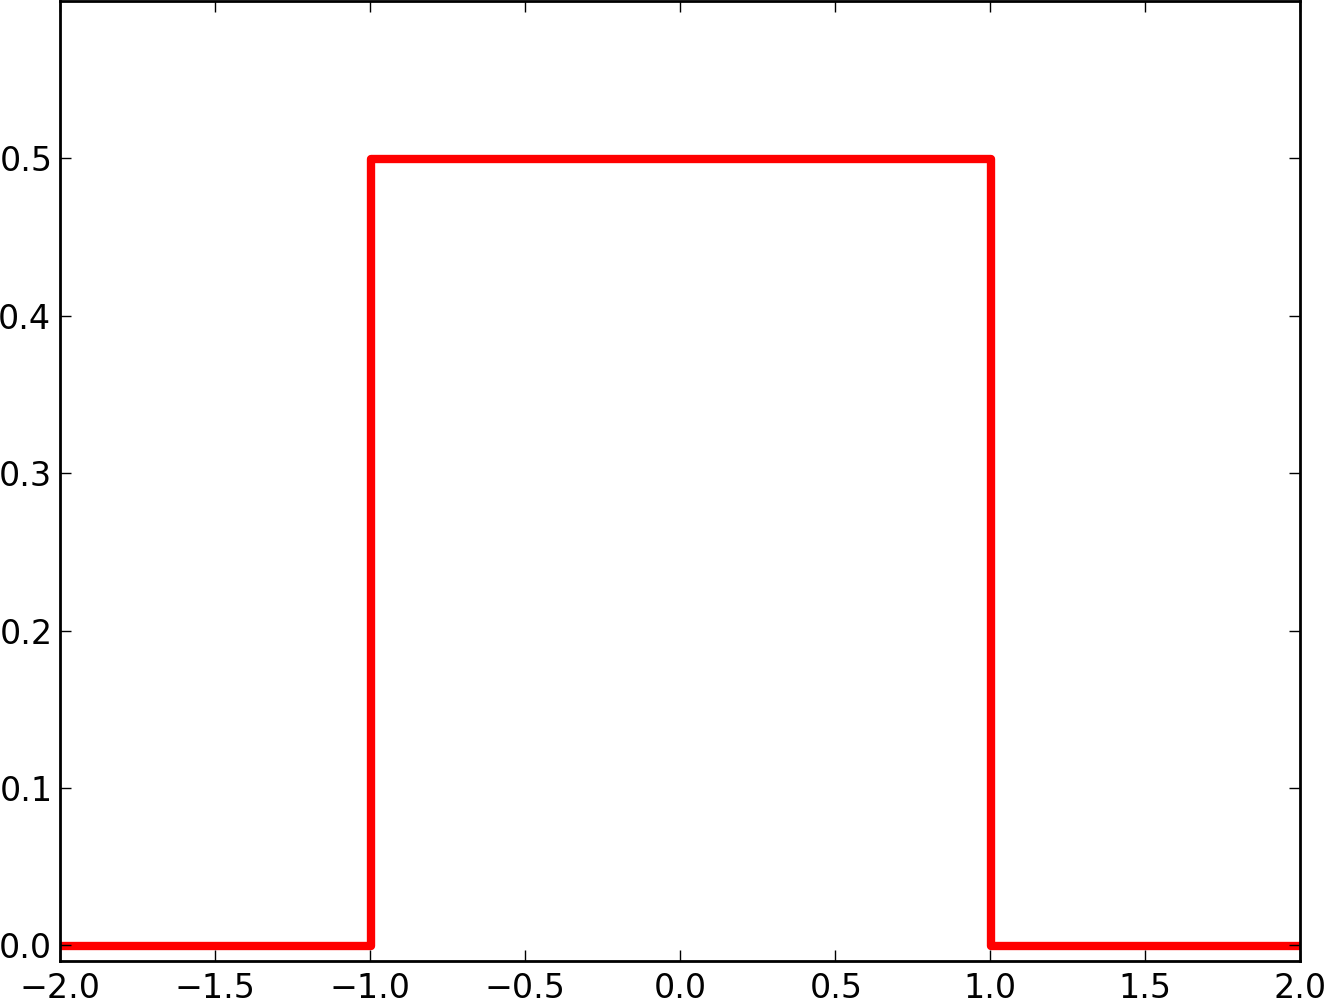
\includegraphics[width=0.9\textwidth]{./fig/fig_unif.png}
\caption{$a=-1$ and $b=1$}
\end{figure}
\end{exampleblock}
\end{columns}
\note{make basics calculations with uniform probability}

\end{frame}


%%%%%%%%%%%%%%%%%%%%%%%%%%%%%%%%%%%%%%%%%%%%%%%%%%%%%%%%%%%%%%%%%%%%%%%%%%%%%%%%%%%%%%
\begin{frame}{An example of joint probability}
Among 27 students who attend a class this day :
\begin{itemize}
\item 6 had a party last night and are still attentive in class 
\item 12 had a party last night and feel too sleepy to be attentive
\item 3 had no party last night but are not attentive in class
\item 6 had no party last night and are attentive in class
\end{itemize}

In term of Probability Mass Function:
\begin{itemize}
\item $N$ is a random variable such as $N=1$ if a random student did have a party and $0$ otherwise.
\item $A$ is a random variable  such as $A=1$ if a random student is attentive and $0$ otherwise.
\end{itemize}
\begin{table}
\centering
\begin{tabular}{|l||c|c|}
\hline
\backslashbox{N}{A} & 0 & 1 \\
\hline \hline
0 & 1/9 & 2/9 \\
\hline
1 & 4/9 & 2/9 \\
\hline
\end{tabular}
\end{table}
\note{Basic calculations (normalization), scheme}
\end{frame}

%%%%%%%%%%%%%%%%%%%%%%%%%%%%%%%%%%%%%%%%%%%%%%%%%%%%%%%%%%%%%%%%%%%%%%%%%%%%%%%%%%%%%%
\begin{frame}
\frametitle{Marginal probability}
\begin{block}{Definition}
Given a set of random variable with a probability distribution $P(X_1,X_2,X_3, \cdots,X_n)$
The marginal probability is the probability distribution over a subset of these variables:
$P(X_1,\cdots,X_p)$ with $p<n$
\end{block}
For two random variables $X$,$Y$:
\begin{itemize}
\item In the discrete case: $P(X=x) = \sum_y P(X=x,Y=y)$
\item In the continous case: $f_X(x) = \int f_{X,Y}(x,y)dy$
\end{itemize}

With the Previous example:
\begin{table}
\centering
\begin{tabular}{|l||c|c|r|}
\hline
\backslashbox{N}{A} & 0 & 1 & $P(N=n)$ \\
\hline \hline
0 & 1/9 & 2/9 & 3/9 \\
\hline
1 & 4/9 & 2/9 & 6/9\\
\hline
$P(A=a)$ & 5/9 & 4/9 & 1 \\
\hline
\end{tabular}
\end{table}
\note{Do a calculation, explain in plain english}
\end{frame}


%%%%%%%%%%%%%%%%%%%%%%%%%%%%%%%%%%%%%%%%%%%%%%%%%%%%%%%%%%%%%%%%%%%%%%%%%%%%%%%%%%%%%%
\begin{frame}
\frametitle{Conditional probability}
\begin{block}{Definition}
A conditional probability is the probability of some event (e.g. $Y=y$) given that
some other event actually happened (e.g. $X=x$). This can be computed given the
formula:
$$
P(Y=y | X=x) = \frac{P(Y=y,X=x)}{P(X=x)}
$$
\end{block}
There are some equivalent formulas if $X$ and/or $Y$ are continous:
\begin{itemize}
\item if both $X$ and $Y$ are continuous: $f_{Y=y|X=x}(y)=\frac{f_{X,Y}(x,y)}{f_X(x)}$
\item if only $X$ is continous: $P(Y=y | X=x) = \frac{f_{X,Y}(x,y)}{f_X(x)}$
\item if only $Y$ is continous: $f_{Y=y|X=x}(y) =  \frac{f_{X,Y}(x,y)}{P(X=x)}$
\end{itemize}
\note{Follow the example: what is the probability of being attentive knowing that the
student has(or not) a party the night before, and the reverse probability (what is the 
probability of having a party the day before knowing he had a party the night before)}

\end{frame}

%%%%%%%%%%%%%%%%%%%%%%%%%%%%%%%%%%%%%%%%%%%%%%%%%%%%%%%%%%%%%%%%%%%%%%%%%%%%%%%%%%%%%%
\begin{frame}{Joint probability and independance}
If two random variables $X$ and $Y$ are independant:
\begin{itemize}
\item In the discrete case: $P(X=x,Y=y)=P(X=x)P(Y=y)$ and therefore  $P(Y=y|X=x)=P(Y=y)$
\item In the coninous case: $f_{X,Y}=f_X(x)f_Y(y)$ and therefore $f_{Y|X=x}(y) = f_Y(y)$.
\end{itemize}
\note{Are the events of being attentive in class and having a party the night before
are independant ?}

\end{frame}

%%%%%%%%%%%%%%%%%%%%%%%%%%%%%%%%%%%%%%%%%%%%%%%%%%%%%%%%%%%%%%%%%%%%%%%%%%%%%%%%%%%%%%


%%%%%%%%%%%%%%%%%%%%%%%%%%%%%%%%%%%%%%%%%%%%%%%%%%%%%%%%%%%%%%%%%%%%%%%%%%%%%%%%%%%%%%
\begin{frame}
\frametitle{Expectation}
\begin{block}{Definition}
Given a function $g$ of a random variable $X$, the \alert{expectation} is  defined as:
\begin{itemize}
\item if $X$ is discrete: $\E[g(X)]=\sum_xg(x)P(X=x)$
\item if $X$ is continous: $\E[g(X)]=\int_x g(x)f_X(x)dx$
\end{itemize}
\end{block}
In particular:
\begin{itemize}
\item $\E[X] = \sum_xxP(X=x)$ (discrete variable)
\item $\E[X]=\int_x xf_X(x)dx$ (continous variable)
\end{itemize}
Intuitively, the expectation gives an idea of the average value to be expected for a
random variable.
\begin{exampleblock}{Linearity}
$$
\E[a.g(X) + b] = a.\E[g(X)] + b
$$
where $a$ and $b$ are scalar.
\end{exampleblock}
\note{Make the calculation for one dice (21/6 = 3.5) and for two dice (7)}

\end{frame}


%%%%%%%%%%%%%%%%%%%%%%%%%%%%%%%%%%%%%%%%%%%%%%%%%%%%%%%%%%%%%%%%%%%%%%%%%%%%%%%%%%%%%%
\begin{frame}
\frametitle{Variance}
\begin{block}{Definition}
Given a function $g$ of random variable $X$, the \alert{variance} is defined as:
$$
\Var(g(X)) = E\left[ (g(X)-\E[g(X)])^2\right] = \E[g(X)^2] - \E[g(X)]^2
$$
\end{block}
In particular:
$$
\Var(X) = E\left[ (X-\E[X])^2\right] = \E[X^2] - \E[X]^2
$$
Intuitively, the variance describes the spread of the value of a random variable
around its average.

Often, the standard deviation is used:
$$
\sigma(X) = \sqrt(\Var(X))
$$ 
Note : if the variable $X$ has a unit (e.g. meter, second, ...) the expectation and
the standard deviation are of the same unit.
\end{frame}

\begin{frame}{Co-variance}

\begin{block}{Definnition}
The covariance between two random variables $X$ and $Y$ is defined by:
$$
\Cov(X,Y) = \E\left[(X-\E[X])(Y-\E[Y])\right]
$$
\end{block}
if we have a random vector $\bm{X}$, the variance-covariance matrix $\bm{C}$ is defined by:
$$
C_{ij} = \Cov(X_i,X_j)
$$
The diagonal elements of $\bm{C}$ give the variance terms.

\end{frame}

%%%%%%%%%%%%%%%%%%%%%%%%%%%%%%%%%%%%%%%%%%%%%%%%%%%%%%%%%%%%%%%%%%%%%%%%%%%%%%%%%%%%%%
\begin{frame}
\frametitle{Gaussian Distribution}
\vspace{-0.5em}
\begin{block}{Definition}
The \alert{normal distribution} or \alert{gaussian distribution} is largely used.
Given, two parameters $\mu$ and $\sigma$, the density function of a random variable $X$
following such a distribution (denoted $X \sim \mathcal{N}(\mu,\sigma)$) is defined as:
$$
f_X(x) = \sqrt{\frac{1}{2\pi \sigma^2}} \text{exp}\left( -\frac{1}{2\sigma^2}(x-\mu)^2\right)
$$
$\mu$ and $\sigma$ are such that: $\E[X]=\mu$ and $\Var[X]=\sigma^2$
\end{block}
\vspace{-0.5em}
\begin{columns}
\column{0.6\textwidth}
\begin{figure}
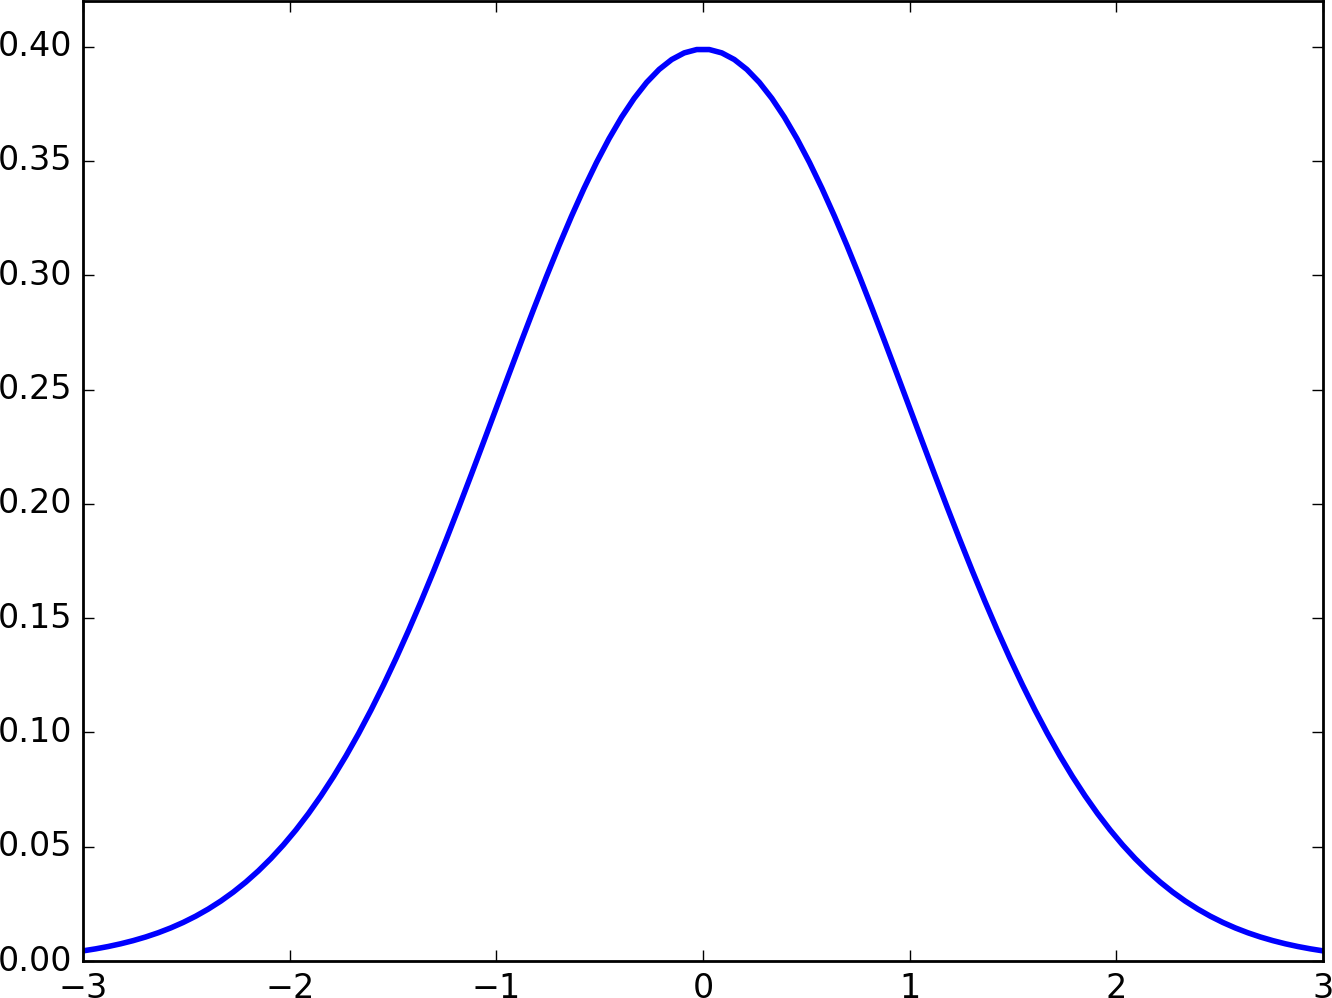
\includegraphics[height=.35\textheight]{./fig/fig_gauss.png}
\end{figure}
\column{0.4\textwidth}
$\mathcal{N}(0,1)$,

Gaussian distribution for $\mu=0$ and $\sigma=1$ called
the \alert{standard normal distribution}.
\end{columns}
\end{frame}
%%%%%%%%%%%%%%%%%%%%%%%%%%%%%%%%%%%%%%%%%%%%%%%%%%%%%%%%%%%%%%%%%%%%%%%%%%%%%%%%%%%%%%
\begin{frame}
\frametitle{Some properties of the gaussian distribution}
\begin{itemize}
\item If $X \sim \mathcal{N}(\mu,\sigma)$. Let's define $X_c=\frac{X-\mu}{\sigma}$. 
We can prove that $X_c \sim \mathcal{N}(0,1)$. This is called \alert{standardization}
\item There is no analytical formula for $P(x \in [a;b])$ except for particular values of $a$
and $b$ ($\{a;b\} \in \{-\infty;0;\infty\}$). So a numeric integration and tabulated values
are used.
\item To give an idea of the spread: $P (-2\sigma < X - \mu < 2\sigma) = 95.45\%$. It means that if 
a random variable follow a normal law, more than 95\% of the realizations (values taken) are
between $-2\sigma$ and $2\sigma$.
\end{itemize}
We can extend this law by defining a multidimensional law on the random vector $\bm{X}$
with the average $\bm{\mu}$ and covariance matrix $\bm{\Sigma}$:
$$
f_{\bm{X}}(\bm{x}) = \sqrt{\frac{\text{det}(\bm{\Sigma}^{-1})}{(2\pi)^n}}
\text{exp}\left(-\frac{1}{2}(\bm{x}-\bm{\mu})^T\bm{\Sigma}^{-1}(\bm{x}-\bm{\Sigma})\right)
$$

\end{frame}

\begin{frame}
\frametitle{Example of one 2-dimensional gaussian}
$\bm{\mu} = (0,0)^T$, $\bm{\Sigma}=\text{Diag}(0.3,0.5)^T$ 
\begin{figure}
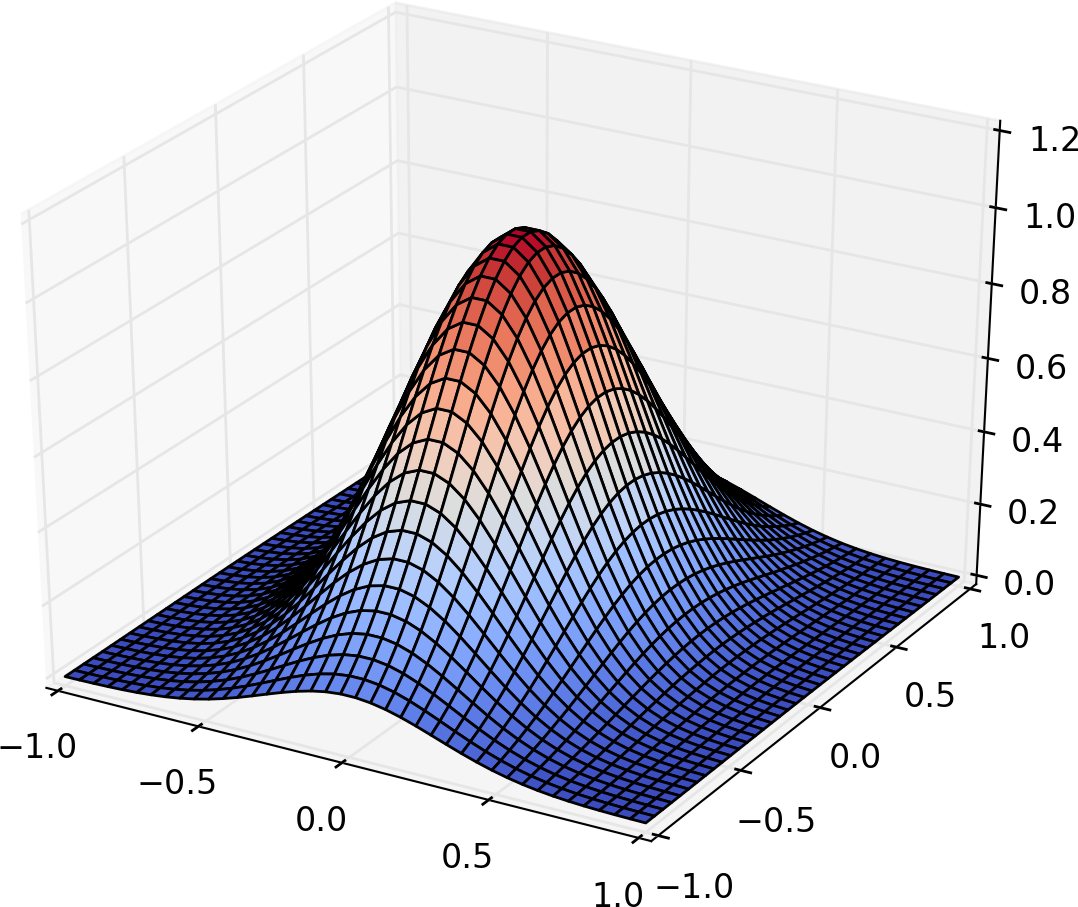
\includegraphics[height=.8\textheight]{./fig/fig_gauss2.png}
\end{figure}
\note{point the axes and remark the difference in spread}
\end{frame}
%%%%%%%%%%%%%%%%%%%%%%%%%%%%%%%%%%%%%%%%%%%%%%%%%%%%%%%%%%%%%%%%%%%%%%%%%%%%%%%%%%%%%%
\begin{frame}
\frametitle{Bayes' Rule}
\begin{alertblock}{}
$$
P(X=x|Y=y) = \frac{P(X=x)P(Y=y|X=x)}{P(Y=y)}
$$
\end{alertblock}
There are equivalent formulation when it involves continous random variables.
For example if $Y$ is continous:
$$
P(X=x|Y=y) = \frac{P(X=x)f_{Y|X=x}(y)}{f_Y(y)}
$$
In practice, it is not needed to calculate $P(Y=y)$, it is possible to use the formula:
$$P(Y=y) = \sum_x P(Y=y|X=x)P(X=x)$$

\note{some quick demonstration + one calculation on a previous example}
\end{frame}


%%%%%%%%%%%%%%%%%%%%%%%%%%%%%%%%%%%%%%%%%%%%%%%%%%%%%%%%%%%%%%%%%%%%%%%%%%%%%%%%%%%%%%
\begin{frame}
\frametitle{Body's temperature and the magic of Bayes' rule}
\framesubtitle{Data of the problem}
\vspace{-0.8em}
\begin{enumerate}
\item Let's consider 2 random variables $X$ and $Y$ related to a randomly picked individual
in the population. $X=1$ if the individual is sick and $0$ otherwise. $Y$ is the random variable
corresponding to his(her) body's temperature.
\item We know the Probability mass function of $X$
\begin{tabular}{|c|c|c|}
\hline
$x$ & 0 & 1 \\
\hline
$P(X=x)$ & 0.9 & 0.1 \\
\hline
\end{tabular}
\item We know the conditional density probablility functions $f_{Y|X=i}(y)$
which are gaussians with mean $\mu_i$ and standard deviation $\sigma_i$.
\end{enumerate}
\vspace{-.5em}
\begin{columns}
\column{0.3\textwidth}
\textcolor[rgb]{0.0, 0.5019607843137255, 0.0}{Healthy:}
\begin{itemize}
\item $\mu_0=37^o$
\item $\sigma_0=0.15^o$
\end{itemize}

\textcolor{red}{Sick:}
\begin{itemize}
\item $\mu_1=38.5^o$
\item $\sigma_1=0.8^o$
\end{itemize}

\column{0.6\textwidth}
\begin{figure}
\centering
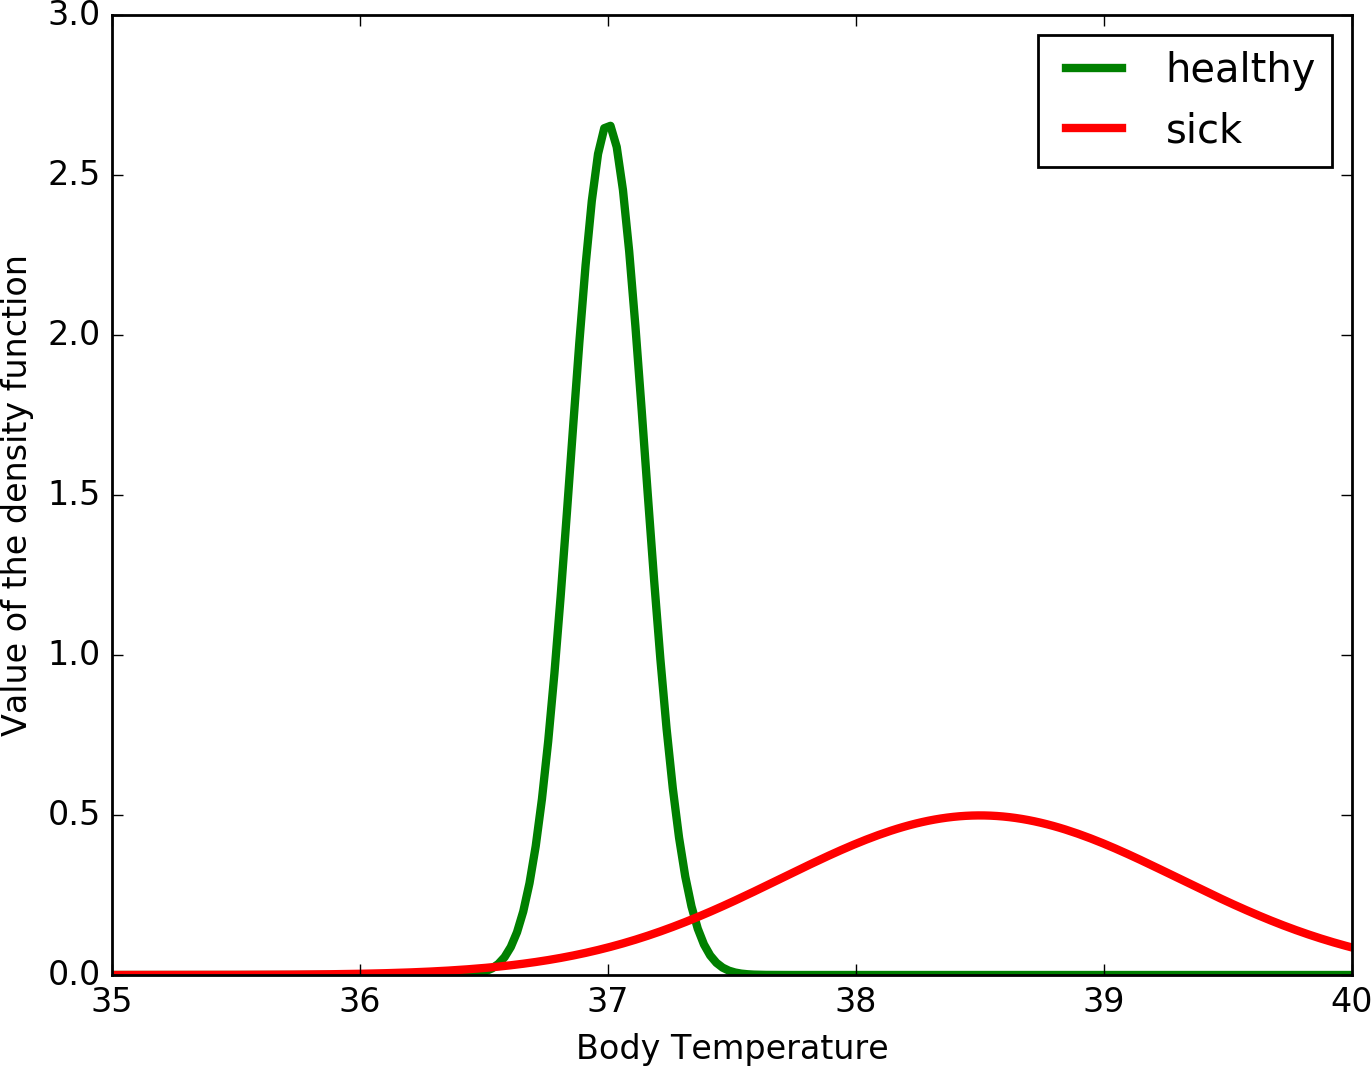
\includegraphics[height=.4\textheight]{./fig/fig_bodyt.png}
\end{figure}

\end{columns}
\end{frame}




%%%%%%%%%%%%%%%%%%%%%%%%%%%%%%%%%%%%%%%%%%%%%%%%%%%%%%%%%%%%%%%%%%%%%%%%%%%%%%%%%%%%%%
\begin{frame}
\frametitle{Body's temperature and the magic of Bayes' rule}
\framesubtitle{What is the question ?}
\begin{block}{}
Given a random person with a body temperature of $y$, what is the probability
of beeing sick ?
\end{block}
Numerical application: $y=37.4^o$

\begin{figure}
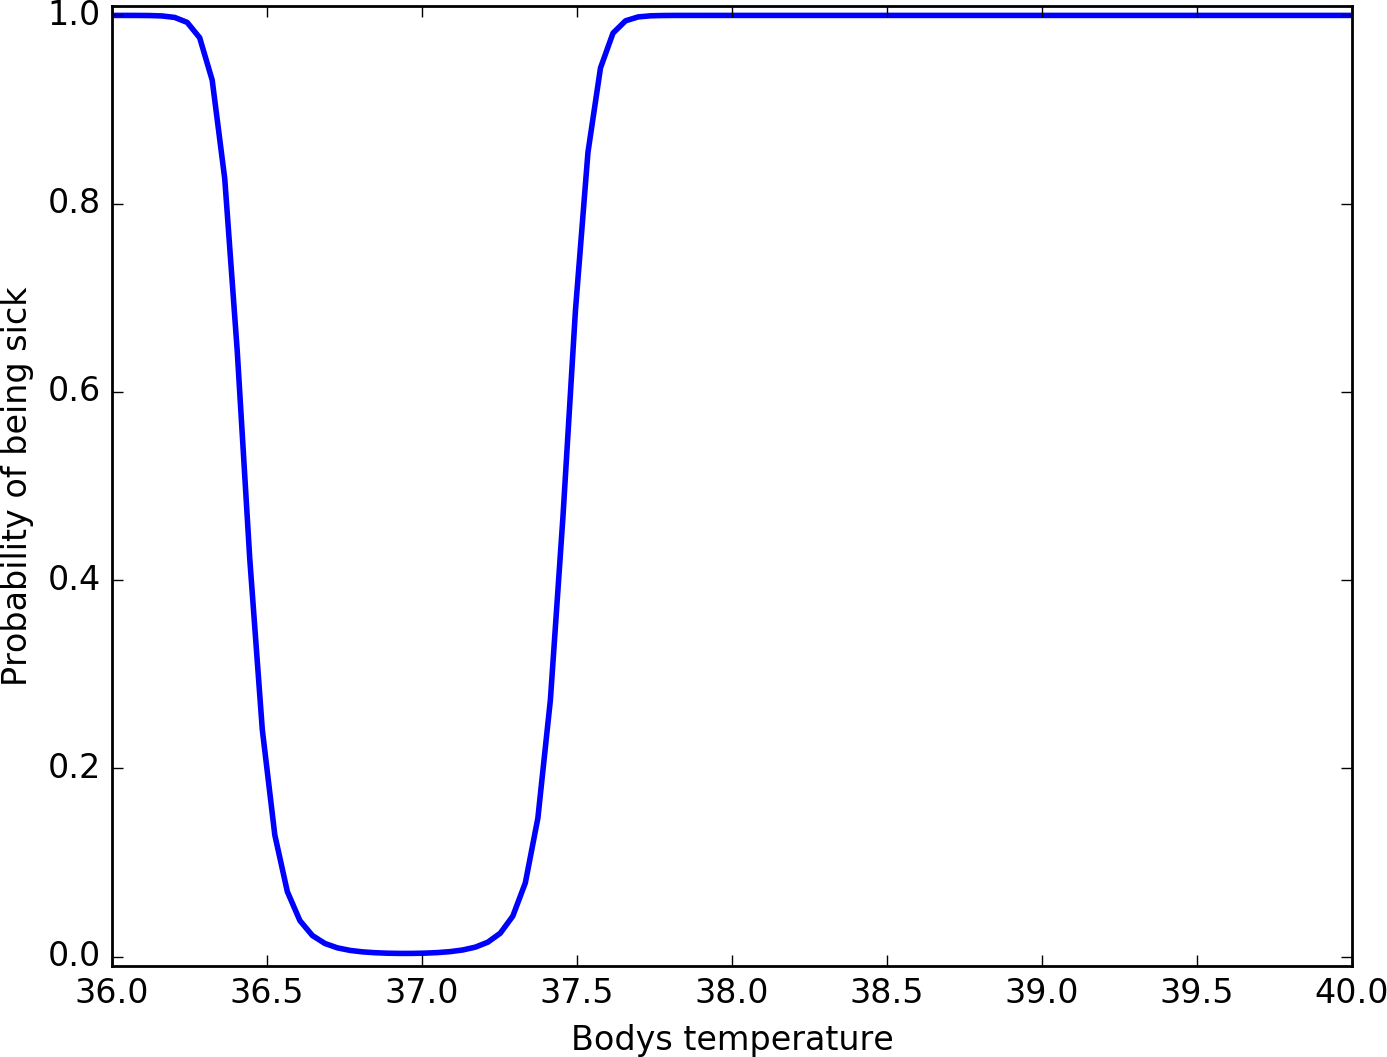
\includegraphics[height=.5\textheight]{./fig/fig_sick.png}
\end{figure}

\note{$P(x=1|y=37.4=0.22)$}



\end{frame}


%%%%%%%%%%%%%%%%%%%%%%%%%%%%%%%%%%%%%%%%%%%%%%%%%%%%%%%%%%%%%%%%%%%%%%%%%%%%%%%%%%%%%%
\begin{frame}
\frametitle{Entropy}
\begin{block}{Definition}
The \alert{shannon entropy} of a discrete random variable $X \sim P(X=x)$ is defined as:
$$
H(X) = -\E[\text{log}(P(X=x))] = - \sum_x P(X=x)\text{log}(P(X=x))
$$
\end{block}
For continuous variable one can use the \alert{Differential entropy}:
$$
h(X) = - \int f_X(x)\text{log}f_X(x)dx
$$
Intuitively, the entropy gives an idea of the surprise expected from a random variable.
A deterministic variable has an entropy of 0.

\note{0log(0)=0}
\end{frame}


%%%%%%%%%%%%%%%%%%%%%%%%%%%%%%%%%%%%%%%%%%%%%%%%%%%%%%%%%%%%%%%%%%%%%%%%%%%%%%%%%%%%%%
\begin{frame}
\frametitle{Example of entropy}
Let's considere a random variable $X$ with two possible values $0$ and $1$.
We note $P(X=1)=p$ and $P(X=0)=1-p$
In this case the entropy is $H(X) = (p-1)\text{log}(1-p) - p \text{log}p$.

\begin{figure}
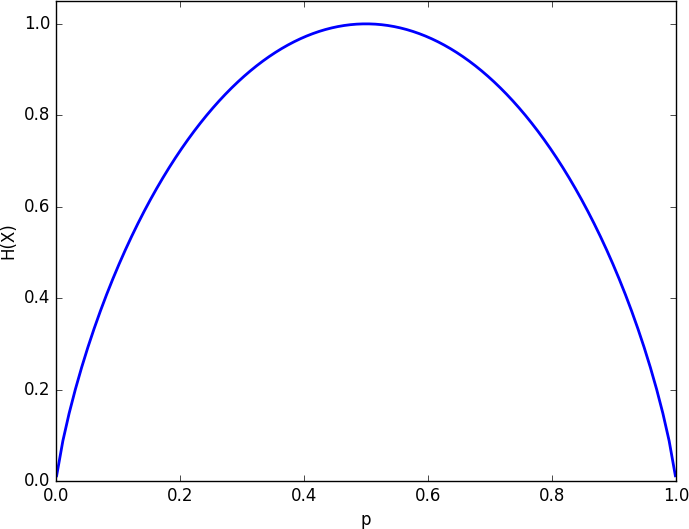
\includegraphics[height=0.6\textheight]{./fig/fig_entropy.png}
\end{figure}
\end{frame}


%%%%%%%%%%%%%%%%%%%%%%%%%%%%%%%%%%%%%%%%%%%%%%%%%%%%%%%%%%%%%%%%%%%%%%%%%%%%%%%%%%%%%%
\begin{frame}
\frametitle{Kullback-Leibler (KL) divergence}
\begin{block}{Definition}
The \alert{The Kullback-Leibler(KL) divergence} is a way to "measure" the difference between 
two probability mass function $P(x)$ and $Q(x)$:
$$
D_{KL}(P\|Q) = \sum_i P(i) \text{log}\frac{P(i)}{Q(i)}
$$
\end{block}
For continuous variables, one can use the definition:
$$
D_{KL}(f_\| f_Y) = \int_x f_X(x) \text{log}\frac{f_X(x)}{f_Y(x)}dx
$$
\textbf{Note:} The divergence is \alert{asymetric}: $D_{KL}(P\|Q) \neq D_{KL}(Q\|P)$

\end{frame}



%%%%%%%%%%%%%%%%%%%%%%%%%%%%%%%%%%%%%%%%%%%%%%%%%%%%%%%%%%%%%%%%%%%%%%%%%%%%%%%%%%%%%%
\begin{frame}
\frametitle{An example}
Let's consider $p(x)$ a given density function (in the example $p$ is a sum of two gaussian).
We want to find the gaussian $q^*(x)$ that minimize the KL divergence.
\begin{figure}
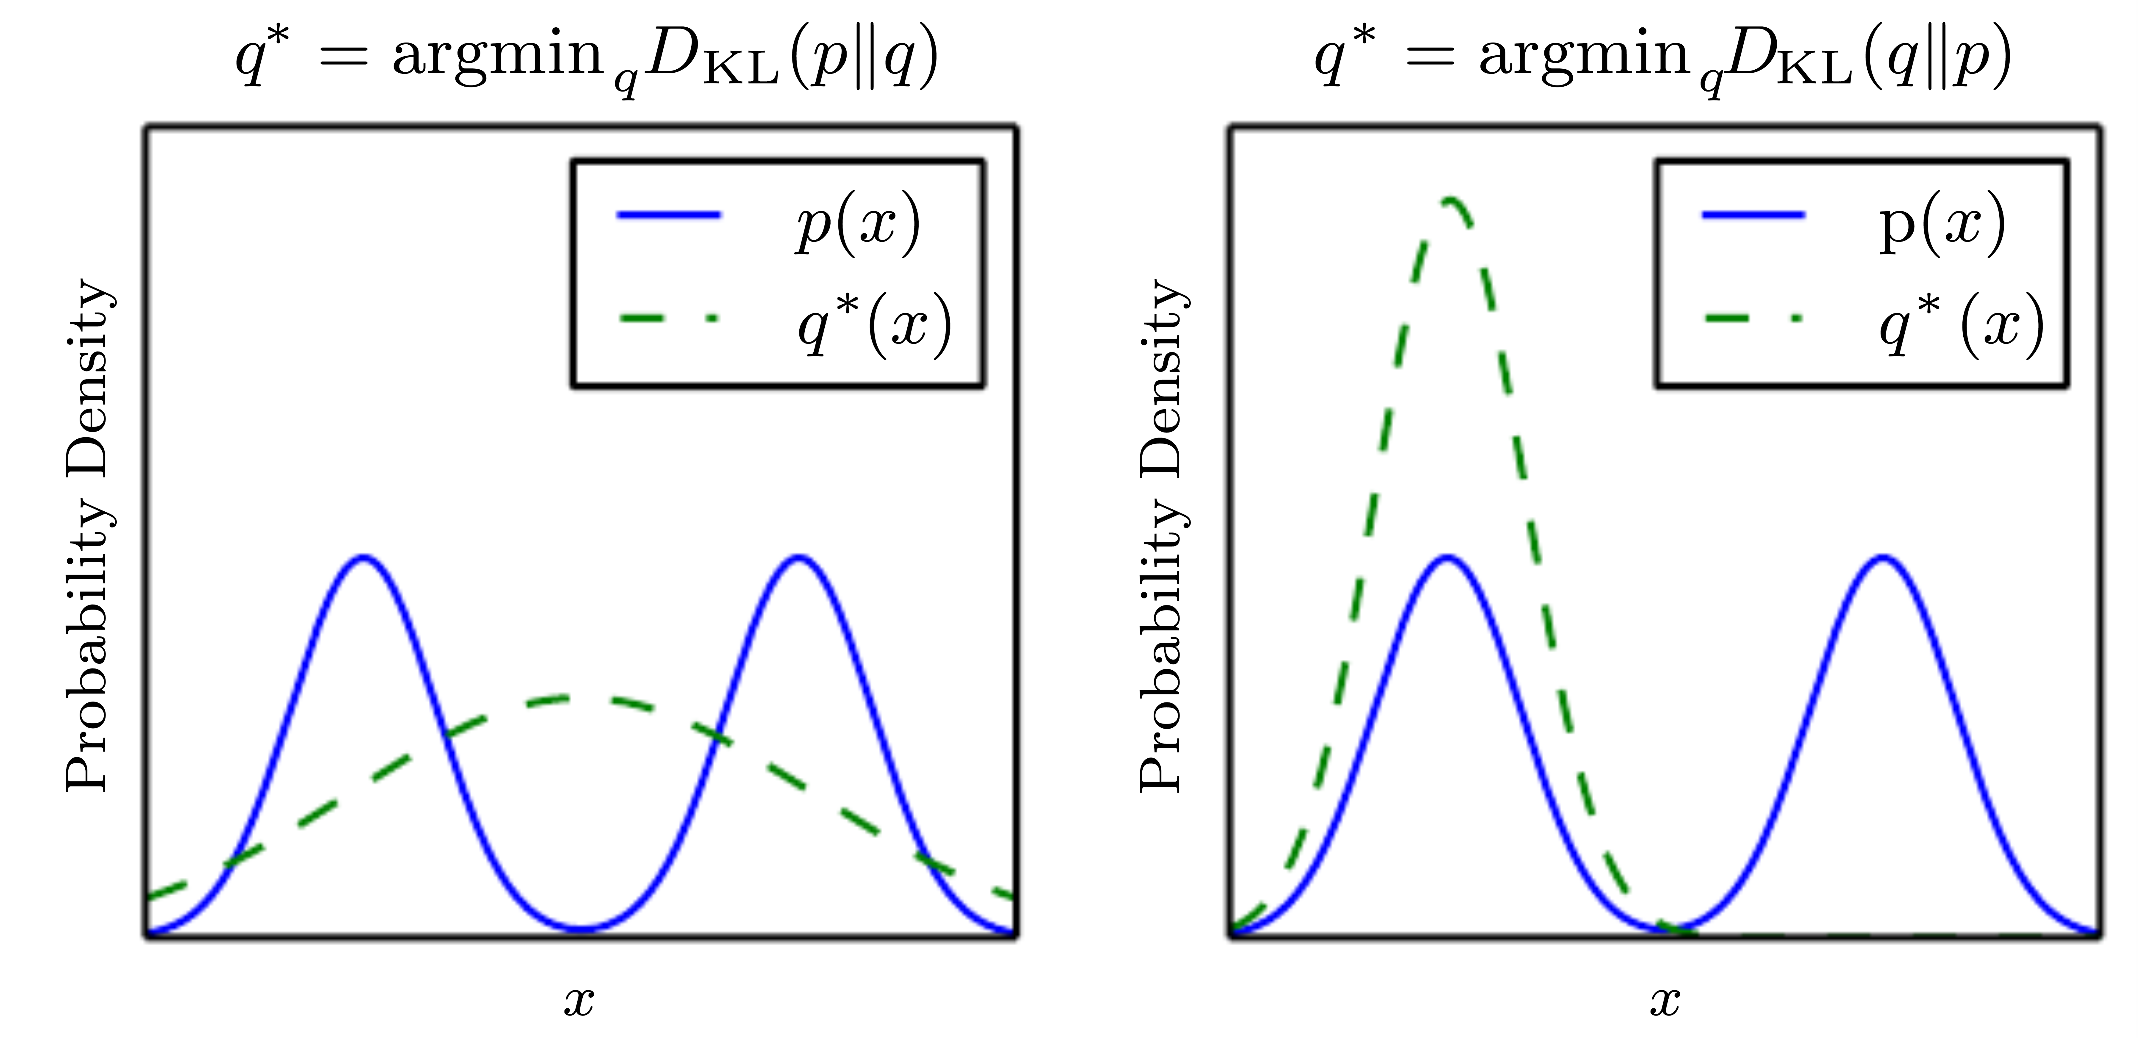
\includegraphics[height=.4\textheight]{./fig/fig_kl.png}\\
\footnotesize{\textit{from Goodfellow et al., Deep Learning, www.deeplearningbook.org}}
\end{figure}
\begin{itemize}
\item if $D_{KL}(p\|q)$ is minimum: $p(x)$ is likely $\Rightarrow$ $q^*(x)$ is likely
\item if $D_{KL}(q\|p)$ is minimum: $p(x)$ is unlikely $\Rightarrow$ $q^*(x)$ is unlikely
\end{itemize}
\end{frame}


%%%%%%%%%%%%%%%%%%%%%%%%%%%%%%%%%%%%%%%%%%%%%%%%%%%%%%%%%%%%%%%%%%%%%%%%%%%%%%%%%%%%%%
\begin{frame}
\frametitle{Cross-entropy}
\begin{block}{Definition}
The cross-entropy of the probability distributions $p$ and $q$ are defined by:
$$
H(p,q) = H(p) + D_{KL}(p\|q)
$$
\end{block}
If $p$ and $q$ are density functions, it gives:
$$
H(p,q) = \int_X p(x) \text{log}q(x) dx
$$

Intuitively, the cross-entropy, is the degree of surprise of a random variable X if we consider
a pratical distribution $q$ different from the true distribution $p$


\end{frame}



%%%%%%%%%%%%%%%%%%%%%%%%%%%%%%%%%%%%%%%%%%%%%%%%%%%%%%%%%%%%%%%%%%%%%%%%%%%%%%%%%%%%%%
\begin{frame}
\frametitle{Sampling}
\begin{block}{Random sample (or independant identically distributed (i.i.d.) random variables)}
Considering a random variable $X$ following a probability distribution.

A \alert{sample}, is a set of $n$ independant random variables $\{X_1,X_2,\ldots,X_n\}$ such as 
each $X_i$ is following the same distribution as $X$.
\end{block}
\begin{block}{Observed values}
In practice, we have access to a particular realization of a random sample denoted
 $\{x_1,x_2,\ldots,x_n\}$
\end{block}
\end{frame}

%%%%%%%%%%%%%%%%%%%%%%%%%%%%%%%%%%%%%%%%%%%%%%%%%%%%%%%%%%%%%%%%%%%%%%%%%%%%%%%%%%%%%%
\begin{frame}
\frametitle{Estimator/Estimate}
Let's denote $\theta$ a parameter of a probabiliy distribution (e.g. $\theta = \mu$, the expectation
of a normal distribtion)
\begin{block}{Definition of an Estimator}
An estimator $\Theta$ is random variable defined as a function of the random variables $\Theta = u(X_1,\ldots,X_n)$ 
that gives a "good estimation" of $\theta$.
\end{block}

\begin{block}{Definition of the point estimate}
A point estimate (often) denoted $\hat{\theta}$ is the function $u$ applied to the observed values
$$
\hat{\theta} = u(x_1,\ldots,x_n)
$$
\end{block}

\end{frame}

%%%%%%%%%%%%%%%%%%%%%%%%%%%%%%%%%%%%%%%%%%%%%%%%%%%%%%%%%%%%%%%%%%%%%%%%%%%%%%%%%%%%%%
\begin{frame}
\frametitle{Example of the Expectation}
\begin{exampleblock}{Estimation of the expectation}
$$
M = \frac{1}{n}\sum_i X_i
$$
where $\{X_1,X_2,\ldots,X_n\}$ is a i.i.d sample, is an estimator of the
expectation $\E(X)$
\end{exampleblock}

\begin{alertblock}{}
Is it a good estimator ?
\end{alertblock}

\end{frame}


%%%%%%%%%%%%%%%%%%%%%%%%%%%%%%%%%%%%%%%%%%%%%%%%%%%%%%%%%%%%%%%%%%%%%%%%%%%%%%%%%%%%%%
\begin{frame}
\frametitle{Properties of an estimator}
Let $\bm{X}=^T(X_1,\ldots,X_n)$ a random sample depending on a parameter $\theta$ and 
$\Theta$ an estimator of $\theta$.\\
Here are some properties of $\Theta$:
\begin{itemize}
\item Mean-square error $\text{MSE}(\Theta) = \E\left[ (\Theta - \theta)^2 \right]$\\
$\text{MSE}(\Theta)$ is espected to be minimum.
\item Bias $B(\Theta) = E(\Theta) - \theta$\\
The bias is expected to be $0$, the estimator is the called \alert{unbiased}
\item $\Theta_n$ (where $n$ denotes the size of the sample) is consistent if and only if:\\
$$\forall \epsilon>0, \lim_{n \to \infty} Pr(|\Theta_n - \theta|<\epsilon)=1$$
\end{itemize}
\end{frame}


\begin{frame}
\frametitle{Example with a normal distribution}
We consider the following estimator of the expectation:
$$
M = \frac{1}{n}\sum_i X_i
$$
we suppose:
$\{X_1,\ldots,X_n\} \sim \mathcal{N}(\mu,\sigma)$
\begin{itemize}
\item $\text{MSE}(M) = \frac{\sigma}{n}$
\item $B(M) = 0$ (no need to make a normal assumption).
\end{itemize}
\note{make the calculation}
\end{frame}


%%%%%%%%%%%%%%%%%%%%%%%%%%%%%%%%%%%%%%%%%%%%%%%%%%%%%%%%%%%%%%%%%%%%%%%%%%%%%%%%%%%%%%
\begin{frame}
\frametitle{Maximum-likelihood estimator}
Knowing a parameter $\theta$, we can compute the following propability:
$$
\mathcal{L}(\theta) = p(x_1,\ldots,x_n | \theta) = p(x_1 | \theta) . p(x_2 | \theta) . \ldots p(x_n | \theta)
$$
$\mathcal{L}$ is called the likelihood.\\

A method to construct an estimator is the construct an estimator that maximimze the likelihood.
In pratice, we use the log-likelihood :
$$
l = \log{\mathcal{L}} = \sum_{i=1}^n \log{p(x_i|\theta)}
$$
\note{Make the calcultion of expectation/Variance with a normal function}

\end{frame}

\end{document}